\section{Prevalence of Fingerprinting Cloaking}
\label{s:prevalence}

\begin{figure}
\centering
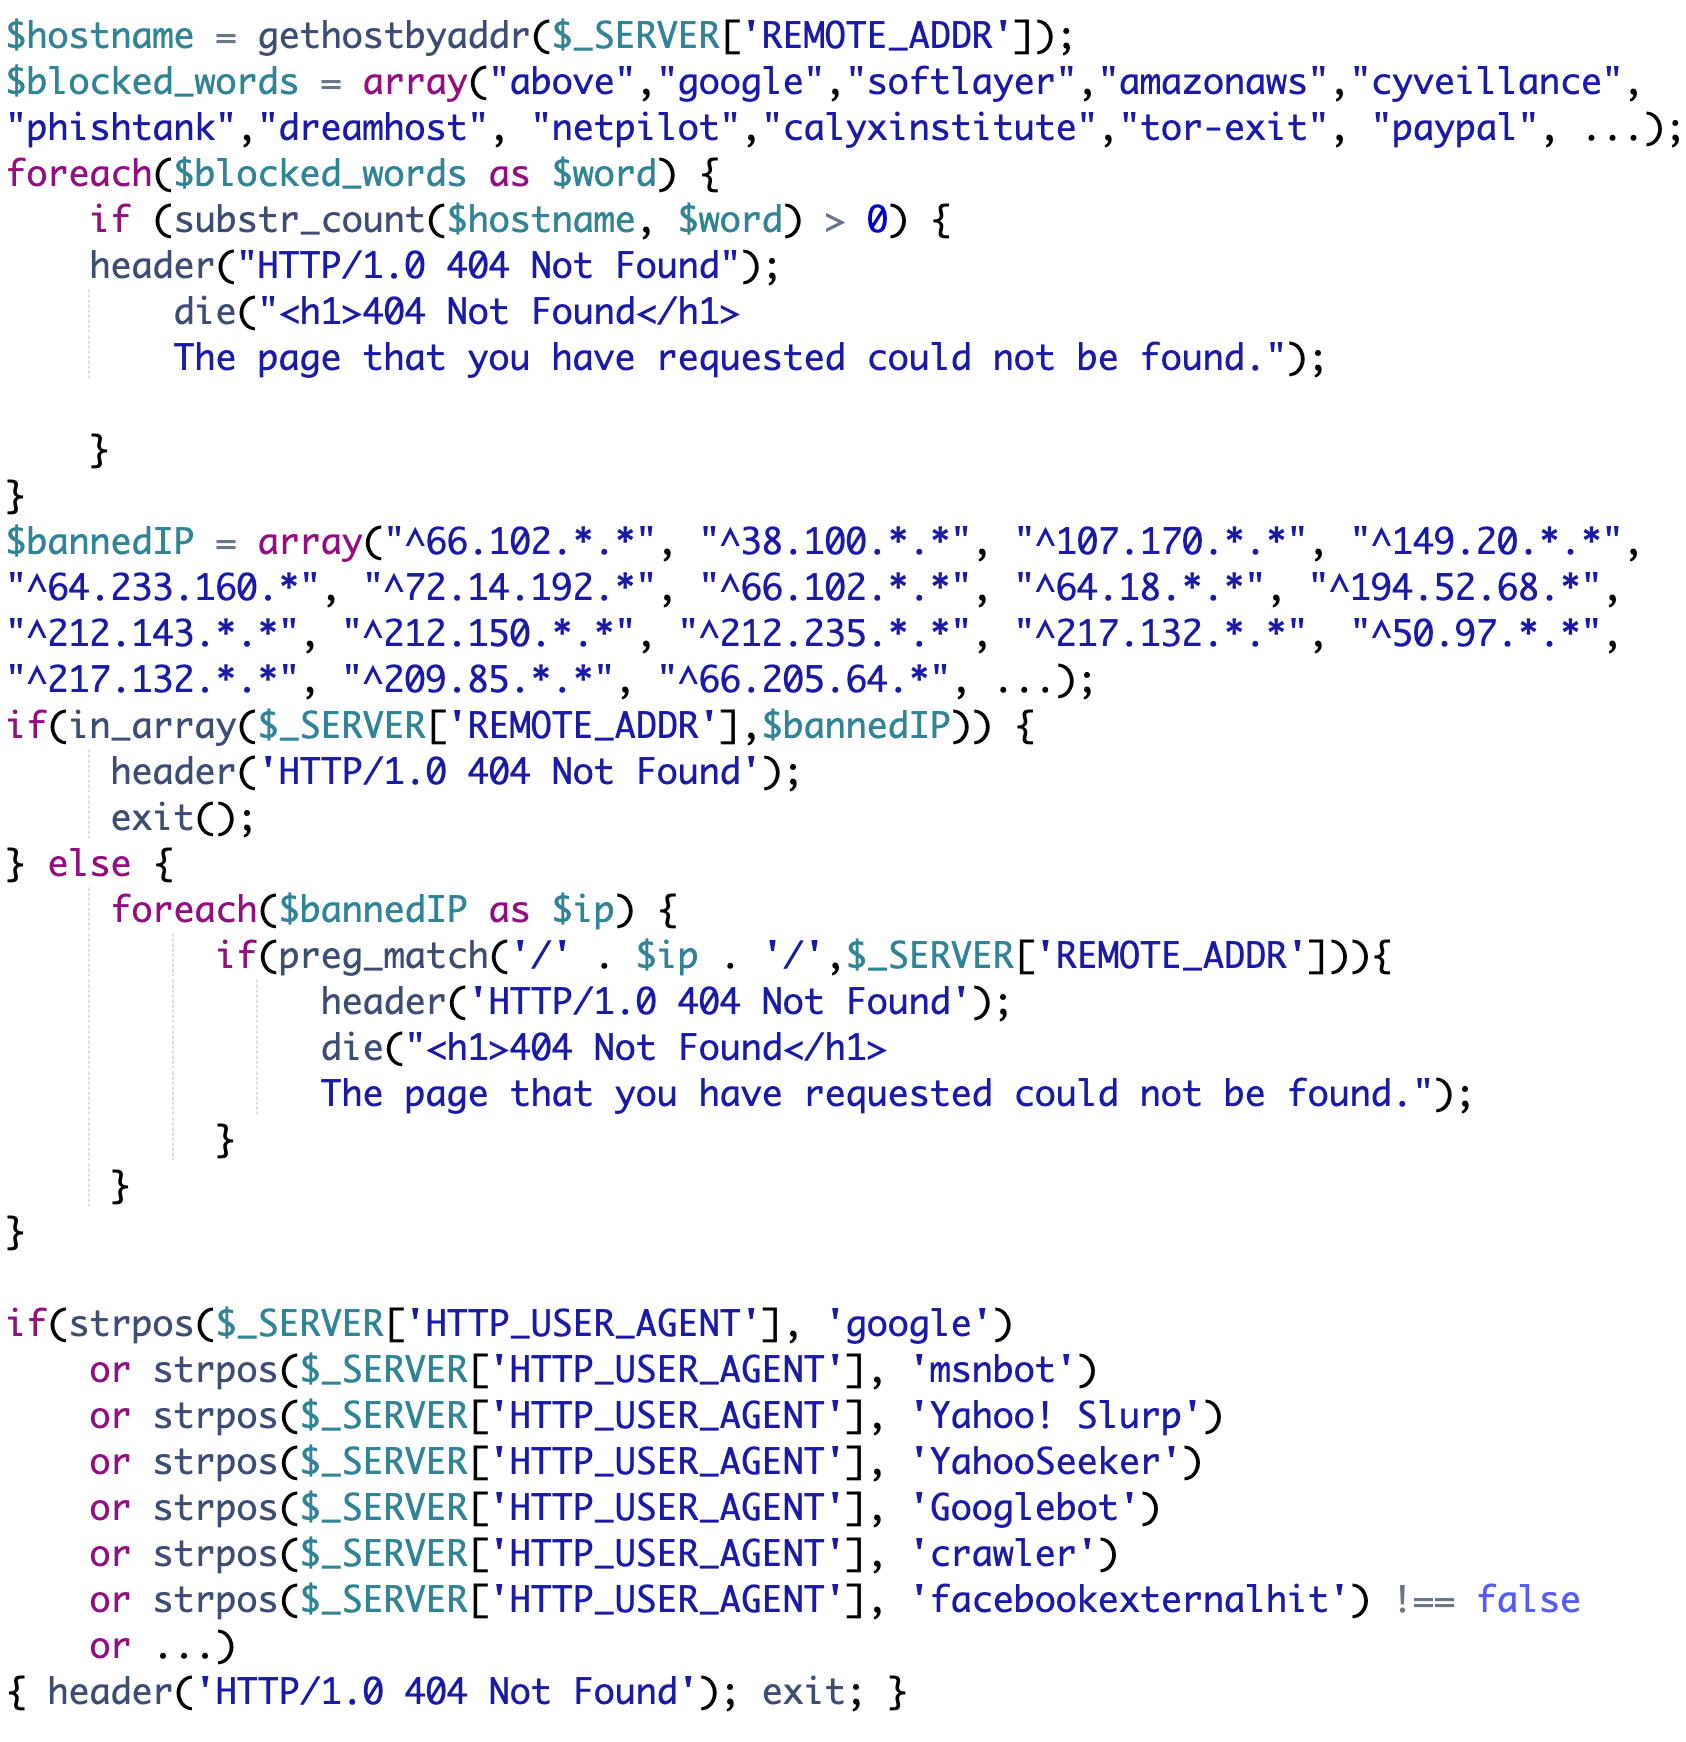
\includegraphics[width=\linewidth]{figs/server_cloaking2.png}
\caption{Simplified PHP code snippet of fingerprinting cloaking in a phishing kit, checking IP, Hostname, and User-Agent.}
\label{fig:servercloaking}
% \vspace{-10pt}
\end{figure}

To understand the prevalence of cloaking techniques used in advanced phishing kits,
we first manually inspect 56 phishing kits, and extract common patterns how fingerprinting cloaking techniques are implemented in phishing kits.

The patterns include (1) sensitive file names such as ``antibot'', ``blocker'', and ``antirobot''; (2) blocked words, for example, an array containing crawler information such as ``google'', ``paypal'', or ``phishtank'' (e.g., \texttt{blocked\_words} in~\autoref{fig:servercloaking}); (3) IP checker that blocks visit from certain IP addresses, such as \texttt{bannedIP} in~\autoref{fig:servercloaking}; and (4) error header, returning an error status code and an error web page, such as \texttt{header} function in PHP.
These attributes reflect the implementation of fingerprinting cloaking techniques in phishing kits.

With these patterns, we can automatically inspect such evasion in phishing kits to evaluate its prevalence.
Among the inspected kits in~\emph{phishunt.io}~\cite{phishunt} from May 2020 to July 2021, \fpphishingkit of \totalphishingkit contain cloaking techniques to fingerprint anti-phishing crawler visit through IP, Referrer, or User-Agent.
To comprehensively measure the prevalence of server-side fingerprinting cloaking techniques in phishing kits,
we also run our pattern finding script on Cisco's dataset that is contributed to Virus Total.
In total, all of 2,421 phishing kits from Cisco's dataset contain such evasion.
Among them, 1,983 of the advanced phishing kits contain User-Agent checker.
% Preliminarily, 100 out of 100 phishing kits from Cisco's dataset contain such evasion.
% , while only one implements server-side click-through cloaking.

From this experiment,
we show that phishers prefer to fingerprint visit through information in HTTP request to distinguish humans out of crawlers.
And thanks to the fact, 
% \spartacus 
we can design a framework to evade phishing websites generated from such advanced phishing kits by triggering the cloaking techniques.



\noindent
\textbf{Popular fingerprinting words.}
To understand the popularity of blocked words such as ``bot'' and ``curl'' that phishing kits use to evade crawler visit,
we collect \numsenswords words in the User-Agent checker of phishing kits and automatically count the appearance of each word in the examined phishing kits.
\autoref{tab:topsenswords} displays the top 10 used sensitive words in the examined phishing kits.
Note that the frequency of some of these words is over the number of phishing kits.
It is because one phishing kits can contain multiple rules to block visit using these words.
Among all the inspected sensitive words, \texttt{bot} has the most appearance.
The result shows that phishers involve those words into the phishing kits to evade visits, whose profile contains any of the words,
A request that contains ``bot'' or ``curl'' is highly likely to be from an automated anti-phishing system.
Potential victim's profile, on the other hand, does not have these words involved~\cite{commonua}.
With the most frequently blocked words in phishing kits, we can use them and trivially trigger the fingerprinting cloaking techniques in sophisticated phishing websites.


\topsenswords